\documentclass[12pt]{article}

    \usepackage{answers}
    \usepackage{setspace}
    \usepackage{graphicx}
    \usepackage{enumitem}
    \usepackage{multicol}
    \usepackage{mathrsfs}
    \usepackage[margin=1in]{geometry} 
    \usepackage{amsmath,amsthm,amssymb}
     
    \newcommand{\N}{\mathbb{N}}
    \newcommand{\Z}{\mathbb{Z}}
    \newcommand{\C}{\mathbb{C}}
    \newcommand{\R}{\mathbb{R}}
    \newcommand{\rto}{\rightarrow\ }
    \newcommand{\Rto}{\Rightarrow\ }
    \newcommand{\lto}{\leftarrow\ }
    \newcommand{\Lto}{\Leftarrow\ }
    \def\xrto{\ensuremath\xrightarrow}
    \def\xRto{\ensuremath\xRightarrow}
    \def\xlto{\ensuremath\xleftarrow}
    \def\xLto{\ensuremath\xLeftarrow}
    \def\rvec{\ensuremath\overrightarrow}
    \def\lvec{\ensuremath\overleftarrow}
    
    \def\mc{\ensuremath\mathcal}
    \def\mf{\ensuremath\mathbf}
    \def\td{\ensuremath\tilde}
    
    \DeclareMathOperator{\sech}{sech}
    \DeclareMathOperator{\csch}{csch}
     
    \newenvironment{theorem}[2][Theorem]{\begin{trivlist}
    \item[\hskip \labelsep {\bfseries #1}\hskip \labelsep {\bfseries #2.}]}{\end{trivlist}}
    \newenvironment{definition}[2][Definition]{\begin{trivlist}
    \item[\hskip \labelsep {\bfseries #1}\hskip \labelsep {\bfseries #2.}]}{\end{trivlist}}
    \newenvironment{proposition}[2][Proposition]{\begin{trivlist}
    \item[\hskip \labelsep {\bfseries #1}\hskip \labelsep {\bfseries #2.}]}{\end{trivlist}}
    \newenvironment{lemma}[2][Lemma]{\begin{trivlist}
    \item[\hskip \labelsep {\bfseries #1}\hskip \labelsep {\bfseries #2.}]}{\end{trivlist}}
    \newenvironment{exercise}[2][Exercise]{\begin{trivlist}
    \item[\hskip \labelsep {\bfseries #1}\hskip \labelsep {\bfseries #2.}]}{\end{trivlist}}
    \newenvironment{solution}[2][Solution]{\begin{trivlist}
    \item[\hskip \labelsep {\bfseries #1}]}{\end{trivlist}}
    \newenvironment{problem}[2][Problem]{\begin{trivlist}
    \item[\hskip \labelsep {\bfseries #1}\hskip \labelsep {\bfseries #2.}]}{\end{trivlist}}
    \newenvironment{question}[2][Question]{\begin{trivlist}
    \item[\hskip \labelsep {\bfseries #1}\hskip \labelsep {\bfseries #2.}]}{\end{trivlist}}
    \newenvironment{corollary}[2][Corollary]{\begin{trivlist}
    \item[\hskip \labelsep {\bfseries #1}\hskip \labelsep {\bfseries #2.}]}{\end{trivlist}}
     
    \begin{document}
     
    % --------------------------------------------------------------
    %                         Start here
    % --------------------------------------------------------------
     
    \title{Further Geometry of Differentiation}%replace with the appropriate homework number
    \author{Dhruv Kohli\\ %replace with your name
    Complex Analysis} %if necessary, replace with your course title
     
    \maketitle
    \begin{enumerate}
        \item Under analytic mapping infinitesimal squares are amplitwisted to infinitesimal squares. C-R equations is symbolic representation of this statement. Cart-Cart form of C-R equations $(f(x,y) = u(x,y)+iv(x,y))$ is:
        \begin{align*}
            \partial_{y}f &= i \partial_{x}f\\
            \epsilon \rto f' \epsilon = \partial_{x}f \epsilon &\Rto f' = \partial_{x}f\\
            i\epsilon \rto f' i\epsilon = \partial_{y}f \epsilon &\Rto f' = -i\partial_{y}f
        \end{align*}
        Polar-Cart form of C-R equations $(f(r,\theta) = u(r,\theta)+iv(r,\theta))$ is:
        \begin{align*}
            dr &= rd\Theta\\
            \partial_{\theta}fd\theta &= i \partial_{r}f dr\\
            &= ir \partial_{r}fd\theta\\
            \partial_{\theta}f &= ir\partial_{r}f\\
            dr e^{i\theta} \rto f' dr e^{i\theta} = \partial_{r}f dr &\Rto f' = e^{-i\theta}\partial_{r}f\\
            ie^{i\theta}rd\theta \rto f' ie^{i\theta}rd\theta = \partial_{\theta}fd\theta &\Rto f' = -(i/z)\partial_{\theta}f
        \end{align*}
        Cart-Polar form of C-R equations $(f(x,y) = R(x,y)e^{i\theta(x,y)})$ is:
        \begin{align*}
            \partial_{y}f = i\partial_{x}f &\Rto \partial_{y}R e^{i\theta}) + iRe^{i\theta} \partial_{y}\theta = i(\partial_{x}R e^{i\theta} + iRe^{i\theta} \partial_{x}\theta)\\
            \partial_{y}R  + iR\partial_{y}\theta &= i\partial_{x}R - R \partial_{x}\theta\\
            \partial_{y}R &= -R\partial_{x}\theta \\
            \partial_{x}R &= R\partial_{y}\theta\\
            f' = \partial_{x}f &= -i\partial_{y}f
        \end{align*}
        Polar-Polar form of C-R equations $(f(r,\theta) = R(r,\theta)e^{i\psi(r,\theta)}$ can be obtained using a similar approach.
        \item If origin centred circles are mapped to vertical lines, larger the circle further to the right is the vertical line, with no restriction on how lines are spaced. The analytic mapping that satisfies this partial information can be obtained as follows - Since analytic mapping is conformal and the lines through the origin are $\perp$ to the circles, these lines must map to horizontal lines.
        \begin{align*}
            &\partial_{r}v = 0, \partial_{\theta}u = 0 \Rto v = v(\theta), u = u(r)\\
            &\partial_{\theta}v(\theta) = r\partial_{r}u(r) = A\\
            &v(\theta) = A\theta + \text{const.}, u(r) = A\ln r + \text{const.}\\
            &f(z) = A\log z + B \qquad \text{where } A\in\R, B\in\C
        \end{align*}
        In general, when concentric circles centred at $c$ are mapped to parallel lines at angle $\phi$, then $z\rto e^{-\phi}g(z+c)$ is the unique $\log$ map upto constants. Note that there can be infinitely many non-analytic mapping exhibiting such behaviour. Since $\log z = \ln r + i(\theta + 2m\pi)$ is analytic as derived above, its derivative is given as $(\log z)' = e^{-i\theta}\partial_{r}\log z = e^{-\theta}/r = 1/z = -(i/z)\partial_{\theta}\log z = -(i/z)i = 1/z$. So, the derivative is independent of $m$ i.e. independent of the branch. This can be seen visually by mapping an infinitesimal vector emanating in a $\perp$ direction from $z$ as shown in figure.:
        \begin{figure}[h!]
            \centering
            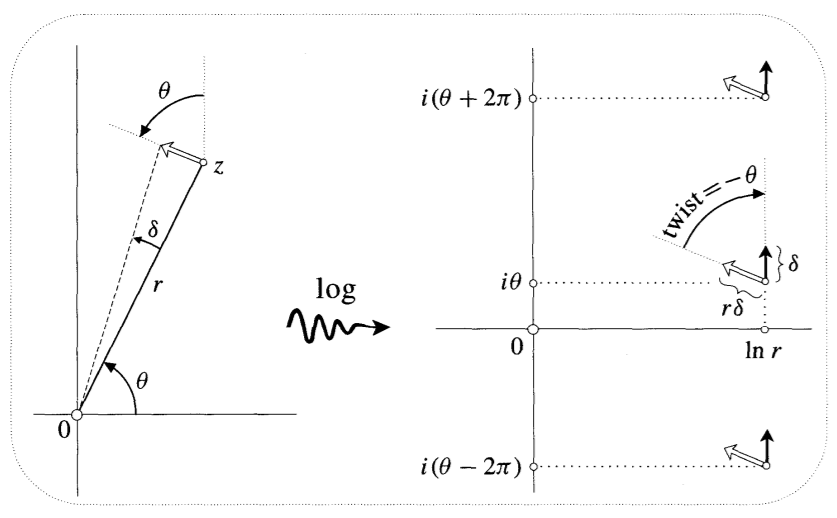
\includegraphics[scale=0.75]{logz}
            \caption{Visual differentiation of $\log z$}
            \label{fig:fig_1}
        \end{figure}
        \item Rules of differentiation: Composition (Note that the functions formed out of these rules are analytic which can be proved visually by computing amplitwists) - If $g$ and $f$ are analytic then so is $g \circ f$ and $(g\circ f(z))' = g'(w)f'(z)$ where $w = f(z)$ which can easily be seen visually (do yourself); Inverse - If $f$ is analytic then so is its inverse. The derivative of inverse at non-critical points is given by $1/f'(z)$ (again see visually yourself); Addition and multiplication - If $f$ and $g$ are analytic then so are $f+g$ and $fg$, and $(f+g)'=f'+g'$ and $(fg)' = f'g + fg'$ (again see visually yourself); Quotient - First note that $I(z) = 1/z$ is conformal and so is analytic and then as visually derived in figure, that $(1/z)' = -1/z^2$ and finally note that, given analytic $g$, $1/g(z) = I \circ g(z)$ which is analytic and by composition rule $(1/g(z))' = -g'(z)/g(z)^2$.
        \begin{figure}[h!]
            \centering
            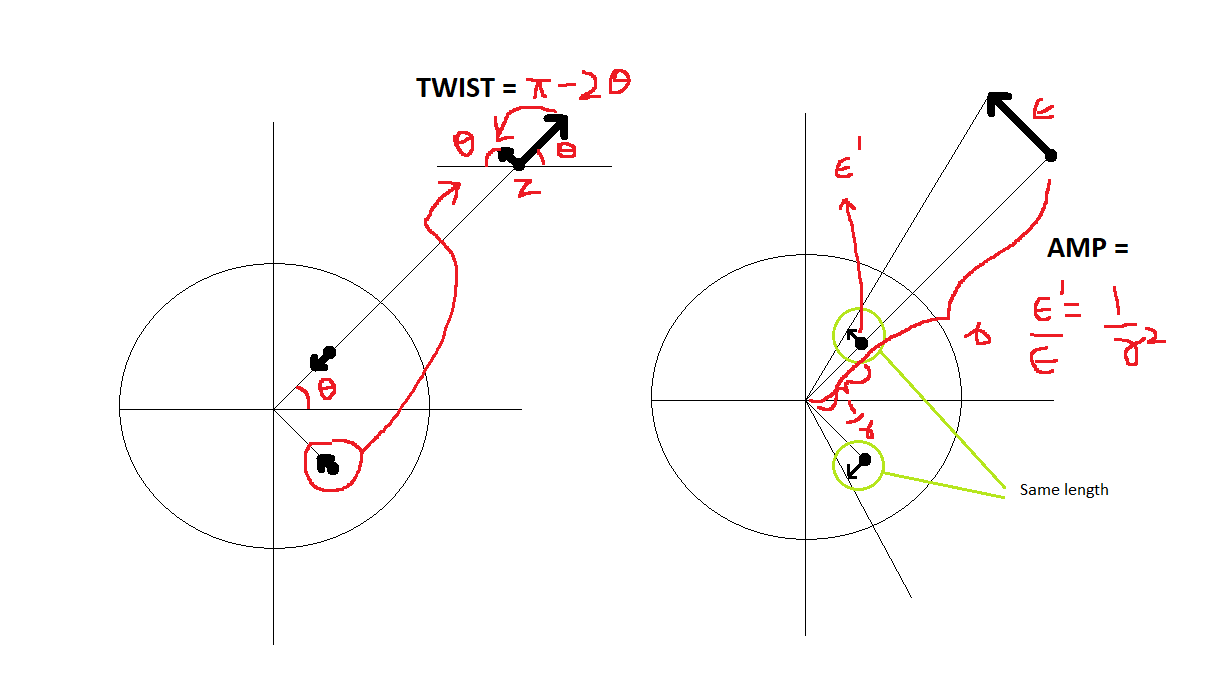
\includegraphics[scale=0.5]{cinv}
            \caption{Visual differentiation of $1/z$}
            \label{fig:fig_2}
        \end{figure}
        \item Polynomials are formed out of the above rules of differentiation, particularly, multiplication and addition, and hence, are analytic. Their derivative can be calculated by computing derivatives term by term. Similarly, rational functions are also analytic $(f(z)/g(z) = f(z)I(g(z)))$ with multiplication, composition and quotient rule in action to form the function and compute its derivative. A power series with a radius of convergence $R$ is also analytic within $R$ by same argument as above. The radius of convergence for its derivative is also $R$ (there is a proof for this) and it is analytic within $R$ too. So, every power series is infinitely differentiable. Any analytic function can be expressed as a power series (proved later) and so any analytic function is infinitely differentiable. This is unlike $\R$ (throw more light upon this?).
        \item $z^a$ is clearly analytic for natural no. as powers (by multiplication rule), for integral powers by quotient rule, for powers of type $1/n$ where $n$ is an integer by inversion rule, for rational powers by composition rule, and for real powers by the fact that geometric effect of real powers can be represented with arbitrary precision by rational powers. The derivative of $z^a$ is given by $az^a/z$ where same branch $z^a$ is used on both sides. Visually differentiation of $z^a$ is as shown in the figure.
        \begin{figure}[h!]
            \centering
            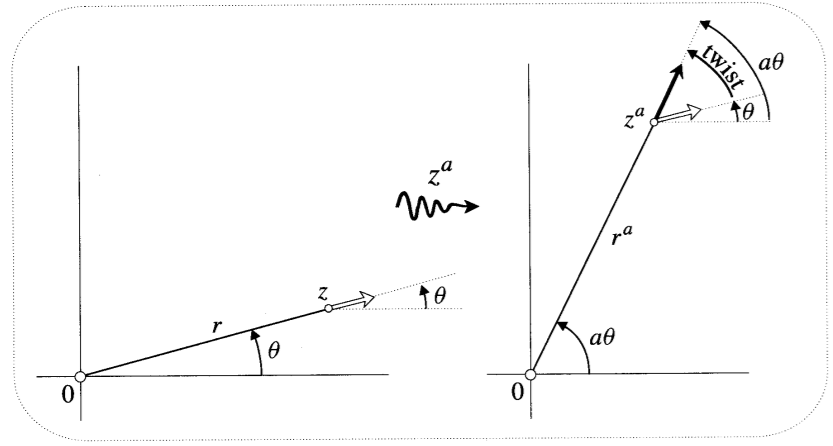
\includegraphics[scale=0.75]{ztpa_1}
            \caption{Visual differentiation of $z^a$}
            \label{fig:fig_3}
        \end{figure}
        \begin{figure}[h!]
            \centering
            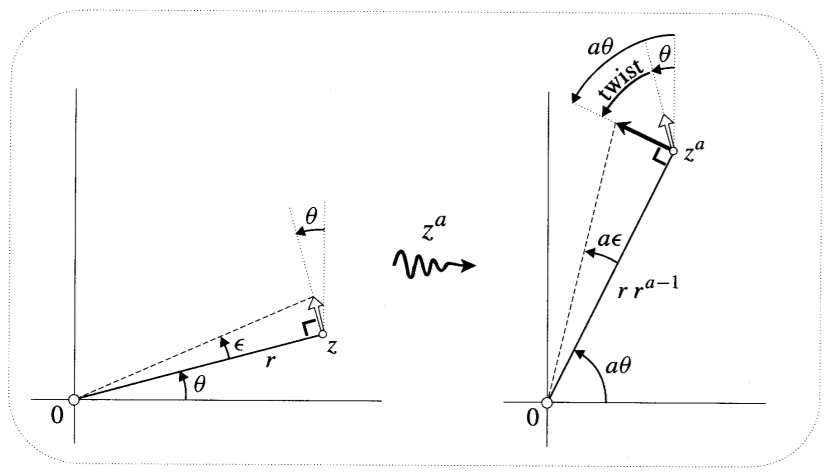
\includegraphics[scale=0.75]{ztpa_2}
            \caption{Visual differentiation of $z^a$}
            \label{fig:fig_4}
        \end{figure}
        \item Visual differentiation of $e^z$ is as shown in the figure.
        \begin{figure}[h!]
            \centering
            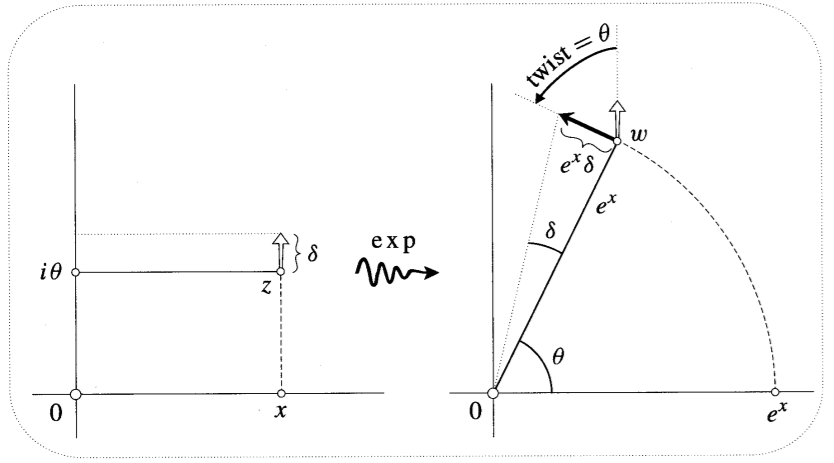
\includegraphics[scale=0.75]{etpz_1}
            \caption{Visual differentiation of $e^z$}
            \label{fig:fig_5}
        \end{figure}
        \begin{figure}[h!]
            \centering
            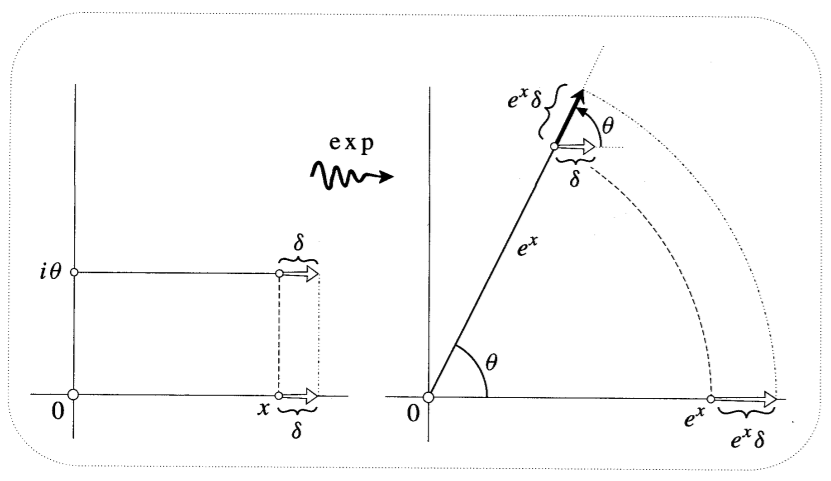
\includegraphics[scale=0.75]{etpz_2}
            \caption{Visual differentiation of $e^z$}
            \label{fig:fig_6}
        \end{figure}
        \item Follow the appropriate figure for the following. If $f$ is analytic then $f$ is infinitely differentiable. So, $f''$ exists. What is the meaning and significance of existence of $f''$? Suppose there is a curve passing through a point $p$ having curvature $\kappa$ at $p$. Then, what is the curvature $\td{\kappa}$ of the image curve under the analytical mapping $f$ at $f(p)$.
        \begin{figure}[h!]
            \centering
            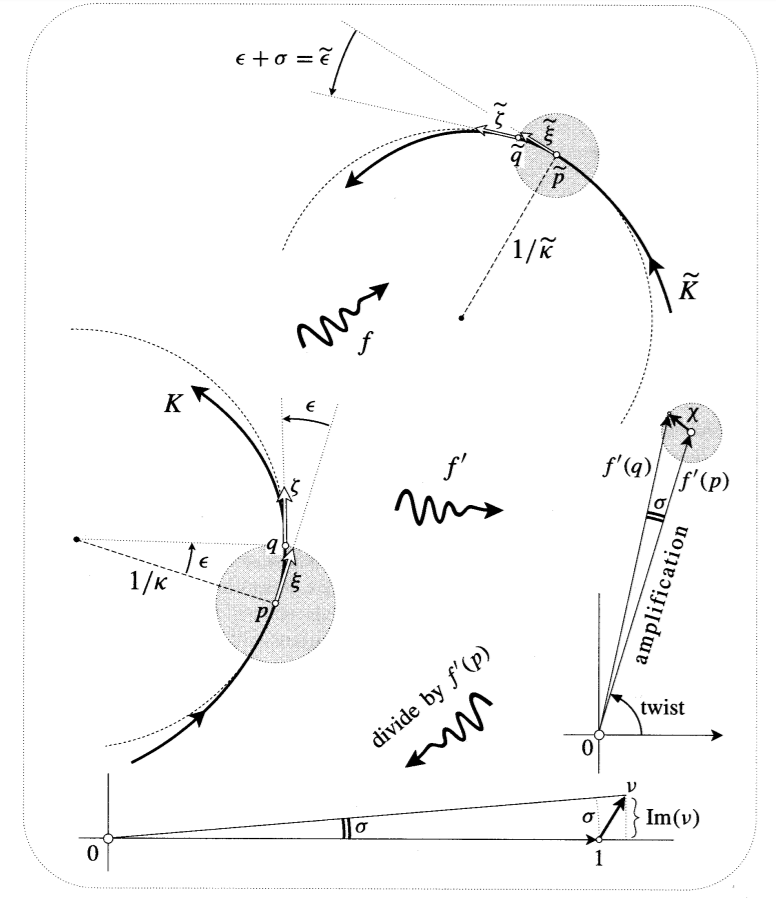
\includegraphics[scale=0.75]{curvature}
            \caption{Computing curvature of image curve at $f(p)$}
            \label{fig:fig_7}
        \end{figure}
        \begin{align*}
            \kappa &= \epsilon/|\xi|\\
            \td{\kappa} &= \td{\epsilon}/|\td{\xi}|\\
            |\td{\xi}| &= |f'(p)||\xi|\\
            \td{\epsilon} &= \epsilon + \sigma\\
            \chi &= f''(p) \xi\\
            \sigma &= \mf{Im}[\chi/f'(p)] = \mf{Im}[f''(p)\xi/f'(p)]\\
            \td{\kappa} &= \mf{Im}[(f''(p)\hat{\xi})/(f'(p)|f'(p)|)] + \kappa/|f'(p)|\\
            \td{\kappa} &= \kappa(\hat{\xi}) + \kappa/|f'(p)|
        \end{align*}
        where $\hat{\xi}$ is a unit vector in the direction of the curvature at $p$. If the a plane containing a circle with radius $R$ centred at origin is expanded by $A$ then the radius of the image circle is $RA$. So, curvature at a point on the circle changes from $1/R$ to $1/(AR)$. In the same way, the term $\kappa/|f'(p)|$ corresponds to change in curvature at $p$ due to the local expansion by $f$. Even if the initial curve has zero curvature, the image curve can then also have a curvature given by $\kappa(\hat{\xi})$ - this is the curvature of the image at $f(p)$ of a straight line passing through $p$ in direction $\hat{\xi}$. None of the two terms are intrinsic to $f$. However, the complex curvature as defined below is intrinsic to $f$,
        \begin{align*}
            \mc{K} &= (i\bar{f''})/(\bar{f'}|f'|)
        \end{align*}
        The projection of $\mc{K}$ emanating from $p$ on a line through $p$ gives the curvature of the image of that line at $f(p)$ i.e.
        \begin{align*}
            \mc{K} \cdot \hat{\xi} &= \mf{Re}[\bar{\mc{K}}\hat{\xi}] = \mf{Im}[i\bar{\mc{K}}\hat{\xi}] = \kappa(\hat{\xi})
            \td{\kappa} &= \mc{K}\cdot \hat{\xi} + \kappa/|f'|
        \end{align*}
        $\mc{K}$ at a point $p$ can be found by computing curvature of the image curve for straight lines in two distinct direction passing through $p$. If $S_1 \equiv \xi$ and $S_2 \equiv i\xi$ are two $\perp$ straight lines passing through $p$ and $\td{\kappa}_1$ and $\td{\kappa}_2$ are the curvatures of the image curves through $f(p)$, then $\mc{K} = \td{\kappa}_1 + i\td{\kappa}_2$ because $\td{\kappa}_1 = \mc{K}\cdot \hat{\xi}$ and $\td{\kappa}_1 = \mc{K}\cdot i\hat{\xi}$ and vector addition of projection in $\perp$ directions reconstructs the vector.
        \item Let $Q$ be an infinitesimal shape and $\td{Q}$ be its image under analytical map $f$. Then $\td{Q}$ rotates most rapidly and its size remains constant when $Q$ moves in the direction of $\mc{K}$. $\td{Q}$ expands most rapidly and does not rotate when $Q$ moves in the direction of $-i\mc{K}$. If $Q$ begins to move in an arbitrary direction $\hat{\xi}$ then the rate of rotation of $\td{Q}$ wrt the the distance that $\td{Q}$ moves is $\mc{R} = \mc{K}.\xi$. Similarly, the rate of expansion of $\td{Q}$ as a fraction to its initial size wrt the distance it moves is given by $\mc{E} = \xi \times \mc{K}$. Proof - As $Q$ translates by $\xi$, $\td{Q}$ not only translates by $f' \xi$ but also rotates and expands. The rotation with respect to original $\td{Q}$ is given by $\sigma = \mathbf{Im}[\chi/f'(p)]$ and expansion wrt to original $\td{Q}$ is given by $\delta = \mf{Re}[\chi/f'(p)]$. Now, $\mc{R} = \sigma/|f'||\xi|$ and $\mc{E} = \delta/|f'||\xi|$. Note that $\sigma$ is maximum when $\chi \perp f' \equiv \xi $ is in direction of $\mc{K}$. Also, $\delta$ is maximum when $\chi || f' \equiv \xi$ is in direction of $-imc{K}$. Finally, we can write the two results in one equation as $\bar{\hat{\xi}}\mc{K} = \mc{R} + i \mc{E}$.
        \begin{figure}[h!]
            \centering
            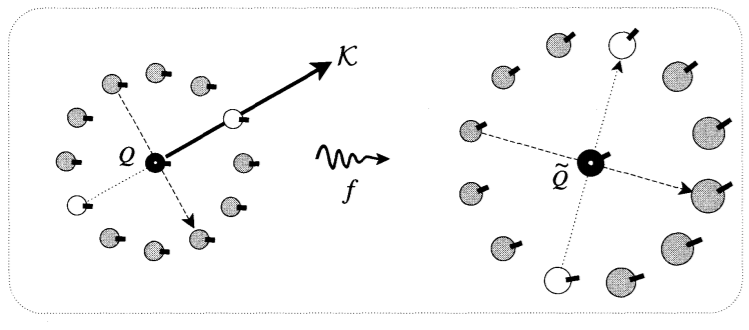
\includegraphics[scale=0.75]{qmotion}
            \caption{Motion of $Q$ and $\td{Q}$}
            \label{fig:fig_5}
        \end{figure}
    \end{enumerate}
    \end{document}
    